\documentclass[11pt]{article}
\usepackage{geometry}                % See geometry.pdf to learn the layout options. There are lots.
\geometry{a4paper}                   % ... or a4paper or a5paper or ... 
%\geometry{landscape}                % Activate for for rotated page geometry
%\usepackage[parfill]{parskip}    % Activate to begin paragraphs with an empty line rather than an indent
\usepackage{graphicx}
\usepackage{amssymb}
\usepackage{amsmath}
\usepackage{lipsum}
\usepackage{authblk}
%\usepackage{amsaddr}
\usepackage{epstopdf}
\usepackage{booktabs}
\usepackage[dvipsnames]{xcolor}
\usepackage{fancyhdr}
\usepackage[yyyymmdd,hhmmss]{datetime}
\pagestyle{fancy}
\rfoot{Compiled on \today\ at \currenttime}
\cfoot{}
\lfoot{Page \thepage}
\RequirePackage[colorinlistoftodos,prependcaption,textsize=tiny]{todonotes} % look for '\todo'
\definecolor{darkred}{rgb}{0.4,0.0,0.0}
\definecolor{darkgreen}{rgb}{0.0,0.4,0.0}
\definecolor{darkblue}{rgb}{0.0,0.0,0.4}
\usepackage[bookmarks,linktocpage,colorlinks,
    linkcolor = darkred,
    urlcolor  = darkblue,
    citecolor = darkgreen]{hyperref}
    
\setcounter{tocdepth}{4}
\setcounter{secnumdepth}{4}

%%%
%%%     Draft margin.
%%%

\usepackage[
    angle=90,
    color=black,
    opacity=1,
    scale=2,
    ]{background}
\SetBgPosition{current page.west}
\SetBgVshift{-4.5mm}
\backgroundsetup{contents={\input{git_information}}}

\usepackage{xspace}
\usepackage{bbm}

%%%%
%%%%    Referring to Parts of the Document
%%%%

\newcommand{\tabref}[1]{Tab.~\ref{tab:#1}\xspace}
\newcommand{\Tabref}[1]{Table~\ref{tab:#1}\xspace}
\newcommand{\figref}[1]{Fig.~\ref{fig:#1}\xspace}
\newcommand{\Figref}[1]{Figure~\ref{fig:#1}\xspace}
\renewcommand{\eqref}[1]{(\ref{#1})\xspace}
\newcommand{\Eqref}[1]{Equation~\ref{eq:#1}\xspace}

%%%%
%%%%    Referring to Other Documents
%%%%

\newcommand{\doi}[1]{\href{http://doi.org/#1}{[#1]}}
\newcommand{\arxiv}[1]{\href{http://www.arxiv.org/abs/#1}{arXiv:#1}}

%%%%
%%%%    Mathematical Symbols
%%%%

\newcommand{\goesto}{\ensuremath{\rightarrow}}
\newcommand{\Integers}{\mathbb{Z}\xspace}
\newcommand{\one}{\ensuremath{\mathbbm{1}}}
\newcommand{\order}[1]{\ensuremath{\mathcal{O}\left(#1\right)}\xspace}
\newcommand{\Rationals}{\mathbb{Q}\xspace}
\newcommand{\Reals}{\mathbb{R}\xspace}
\newcommand{\union}{\ensuremath{\cup}}

%%%%
%%%%    Hyperbolic Trig
%%%%

% Most are already available if you \usepackage{amsmath}.
% However, those below are missing

\DeclareMathOperator{\sech}{sech}
\DeclareMathOperator{\csch}{csch}
\DeclareMathOperator{\arccosh}{arccosh}
\DeclareMathOperator{\arcsinh}{arcsinh}
\DeclareMathOperator{\arctanh}{arctanh}
\DeclareMathOperator{\arcsech}{arcsech}
\DeclareMathOperator{\arccsch}{arccsch}
\DeclareMathOperator{\arccoth}{arccoth}

% Additionally, there are some missing trig functions:

\DeclareMathOperator{\arcsec}{arcsec}
\DeclareMathOperator{\arccot}{arccot}
\DeclareMathOperator{\arccsc}{arccsc}

%%%%
%%%%    Mathematical Delimiters
%%%%
\newcommand{\abs}[1]{\ensuremath{\left| #1 \right|}\xspace}
\newcommand{\magnitude}{\abs}
\newcommand{\average}[1]{\ensuremath{\left\langle #1 \right\rangle}\xspace}

% Quantum mechanics bra-ket notation:
\newcommand{\ket}[1]{\ensuremath{\left|\;#1\;\right\rangle}}
\newcommand{\bra}[1]{\ensuremath{\left\langle\;#1\;\right|}}
\newcommand{\bracket}[2]{\ensuremath{\left\langle\;#1\;\middle|\;#2\;\right\rangle}}
\let\braket\bracket


%%%%
%%%%    Physical Quantities and Constants
%%%%




%%%%
%%%%    Software
%%%%

\newcommand{\bash}{\texttt{bash}\xspace}
\newcommand{\git}{\texttt{git}\xspace}
\newcommand{\make}{\texttt{make}\xspace}
\newcommand{\mpi}{\texttt{MPI}\xspace}
\newcommand{\python}{\texttt{python}\xspace}

% Put an xspace after \LaTeX:
\let\builtinLaTeX\LaTeX
\def\LaTeX{\builtinLaTeX\xspace}
 % input rather than include so we don't create macros.aux


%\DeclareGraphicsRule{.tif}{png}{.png}{`convert #1 `dirname #1`/`basename #1 .tif`.png}

\renewcommand{\headrulewidth}{0pt}
%\fancyhead[L]{
%\includegraphics[width=4cm]{/Users/tomluu/Research/talks/fzjTemplate/uniBonn_logo.jpg}
%}
%\fancyhead[R]{
%\includegraphics[width=4cm]{/Users/tomluu/Research/talks/fzjTemplate/fzj_logo.jpg}
%}
\pagestyle{plain}

\title{L\"uscher's formula in 3, 2, 1 (lift off!) dimensions}
\author[1]{Evan Berkowitz}
\author[1,2]{Thomas Luu}
\affil[1]{Institute for Advanced Simulation 4\\
Forschungszentrum J\"ulich, Germany}
\affil[2]{Rheinische Friedrich-Williams-Universit\"at Bonn, Germany}

%\email{t.luu@fz-juelich.de}
\date{}                                           % Activate to display a given date or no date


\begin{document}
\maketitle
\begin{center}
email: \href{mailto:t.luu@fz-juelich.de}{t.luu@fz-juelich.de}
\end{center}
\abstract{
We derive L\"uscher's formula for a torus in 3, 2, and 1 dimensions.
}

\thispagestyle{fancy}

\clearpage{}
%\tableofcontents
%\newpage

\section{Setup}
We consider two interacting particles of equal mass $m$.  We assume a pure contact interaction (regulated if needed depending on dimension),
\begin{equation}
V(\vec{r})=C_0(\Lambda)\delta(\vec{r})\ ,
\end{equation}
where $\vec{r}$ represents the relative distance between the two particles and $C_0(\Lambda)$ is the strength of interaction that in principle depends on the regulator and whose units depend on the spatial dimension $d$.  We also assume the system has zero CM motion (i.e. $\vec{P}_{cm}=0$) to make the problem simpler. The relevant diagram to calculate, both for infinite and finite volume, is the bubble sum shown in \autoref{fig:bubbleSum}:
\begin{figure}[h!]
\center
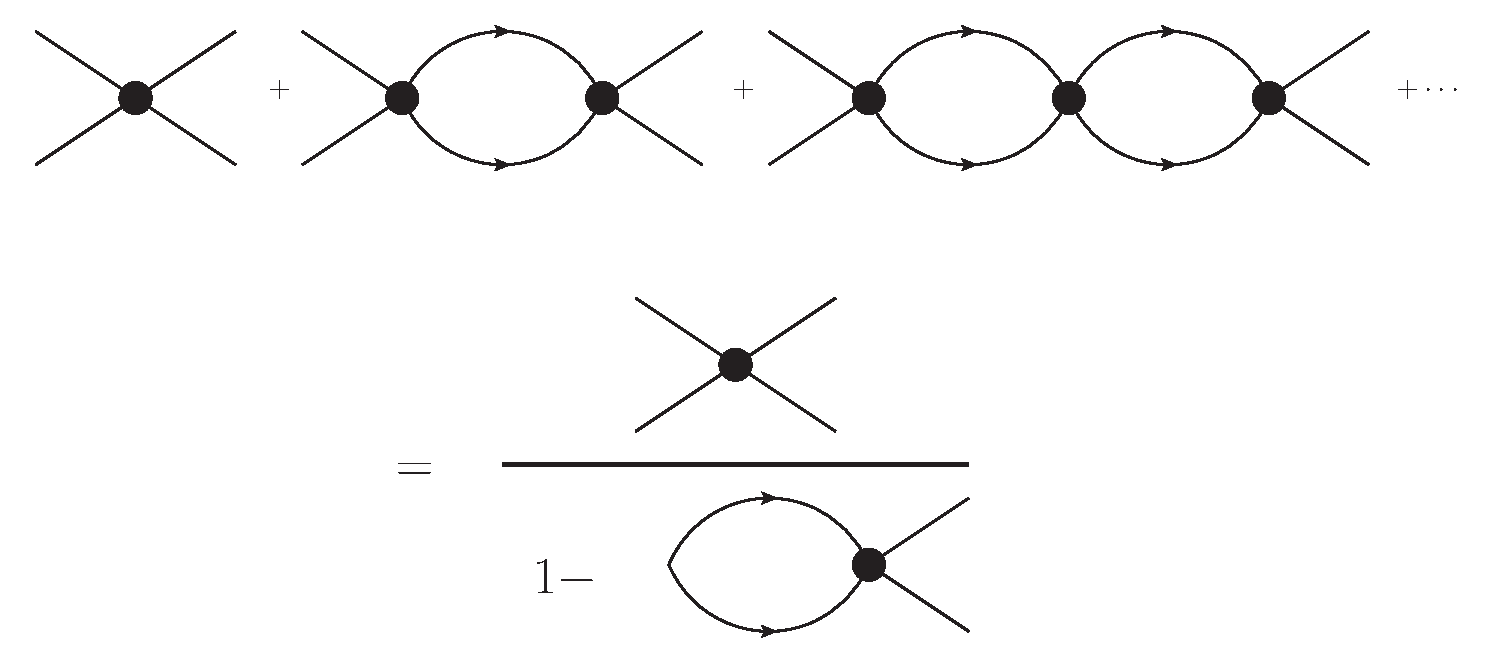
\includegraphics[width=.8\columnwidth]{figure/bubbleSum.eps}
\caption{Bubble sum. Each vertex represents $-iC_0$ and the bubble represents $I_0$.\label{fig:bubbleSum}}
\end{figure}

\noindent The sum is a geometric series and gives\footnote{Note that the {\color{red} red} minus sign in eq.~\eqref{eqn:scattering amplitude} is missing in the archive version of \cite{Beane:2003da}, but is present in \cite{Kaplan:1998we}.}
\begin{equation}\label{eqn:scattering amplitude}
\frac{{\color{red}-}iC_0(\Lambda)}{1-I_0(p,\Lambda)C_0(\Lambda)}\equiv iT(p)\ ,
\end{equation}
where $T$ is the standard T-matrix, $p$ is the relative momentum,  and $I_0(p,\Lambda)$ is a $d$-dependent function (more on this later).  Since we assume a momentum-independent contact interaction, this problem only affects s-wave systems, and the T-matrix in $d$ spatial dimensions can be related to the s-wave phase shift $\delta_0$ by
\begin{equation}
T=\frac{4}{m}\mathcal{F}_d\frac{1}{\cot \delta_0(p)-i}\ ,
\end{equation}
where
\begin{equation}
\mathcal{F}_d=
\begin{cases}
\pi/p & (d=3)\\
1 & (d=2)\\
p/2 & (d=1)
\end{cases}\ .
\end{equation}
Therefore we have
\begin{equation}\label{eqn:T matrix matching}
\boxed{
\frac{4}{m}\mathcal{F}_d\frac{1}{\cot \delta_0(p)-i}=\frac{-C_0(\Lambda)}{1-I_0(p,\Lambda)C_0(\Lambda)}
}\ .
\end{equation}
We can recast eq.~\eqref{eqn:T matrix matching},
\begin{equation}\label{eqn:matching}
\cot \delta_0(p)-i=\frac{4}{m}\mathcal{F}_d\left(\frac{-1}{C_0(\Lambda)}+I_0(p,\Lambda)\right)\ .
\end{equation}
For the special case of a delta function interaction, one has \cite{busch1998}
\begin{equation}\label{eqn:phase shifts}
\cot \delta_0(p) = 
\begin{cases}
 - \frac{1}{a _ { 0 }p }&\quad d=3  \\ 
\frac { 2 } { \pi } \log \left( p a _ { 0 } \right) & \quad d=2\\ 
 p a _ { 0 } &\quad d=1
 \end{cases}\ ,
\end{equation}
where $a_0$ is the scattering length. \autoref{fig:phaseShifts} plots these phase shifts for the different dimensions.  For $d=1,2$ the phase shift asymptotes to zero as $pa_0\to\infty$, while for $d=3$ the phase shift asymptotes to $\pi/2$, corresponding to the (unphysical) fact that the delta function interaction is `felt' at all momentum scales\todo{But the delta function is felt at all momenta in $d=1,2$ cases too, right?}.
\begin{figure}
\center
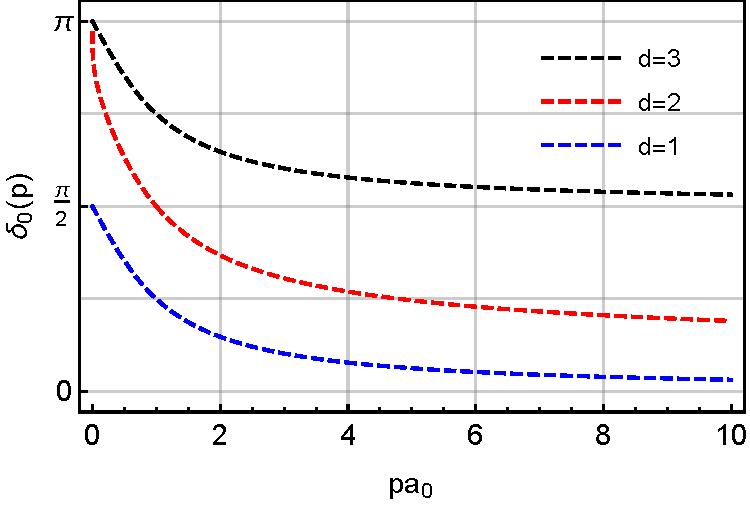
\includegraphics[width=.8\columnwidth]{figure/phaseShift.pdf}
\caption{Phase shift $\delta(p)$, modulo $\pi$, as a function of $pa_0$ for the contact interaction in different dimensions $d$. \label{fig:phaseShifts}}
\end{figure}

%\newpage
\subsection{Infinite volume $I_0$}
Consider the following diagram defining $I_0$:
\begin{figure}[h!]
\center
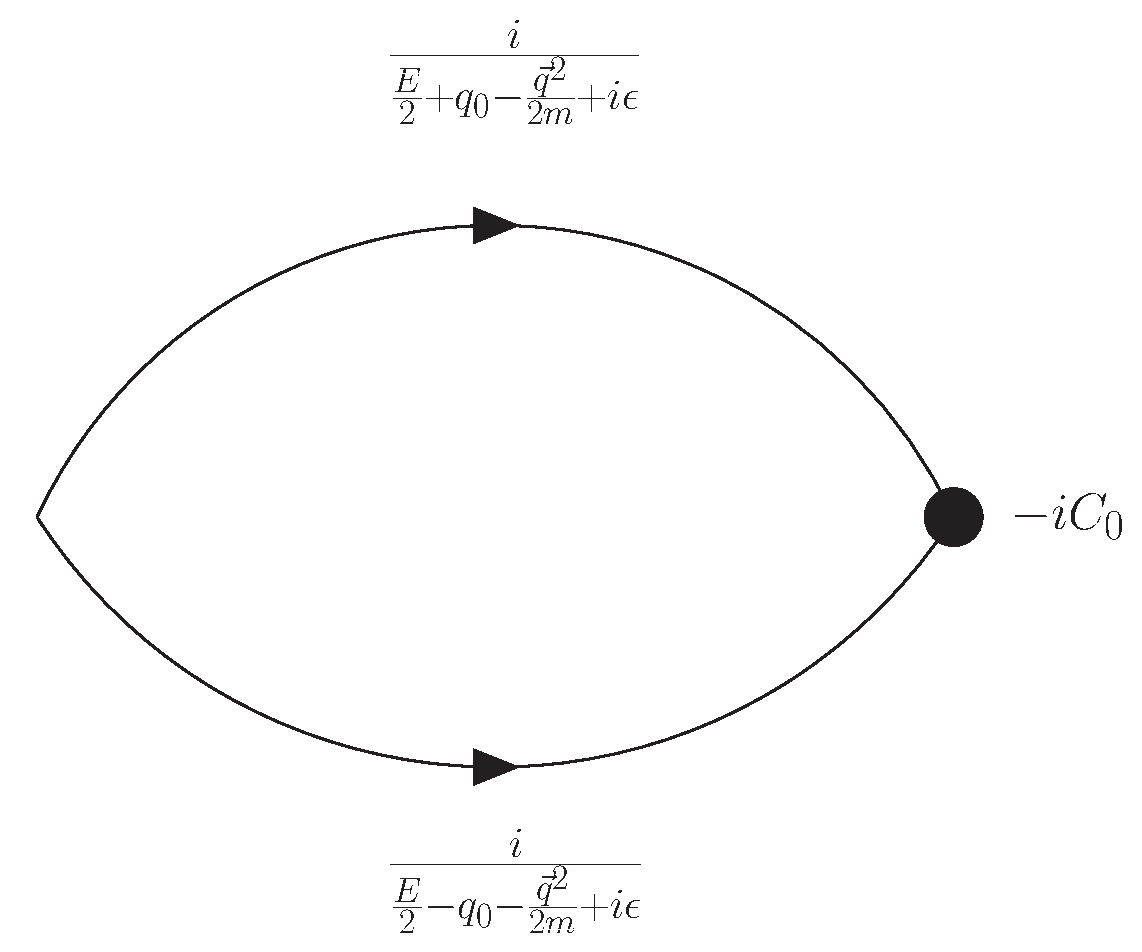
\includegraphics[width=.5\columnwidth]{figure/I0.eps}
\caption{Loop diagram contributing to $I_0$.\label{fig:I0}}
\end{figure}

\noindent The loop integral with $E=p^2/m$ (on-shell relation) gives
\begin{multline}\label{eqn:I0 general}
I_0(p)=-i\int^\Lambda \frac { \mathrm {d}q_0 \mathrm { d } ^ { d } \mathbf { q } } { ( 2 \pi ) ^ { d+1 } } \left( \frac { i } { \frac{E}{2} + q _ { 0 } - \frac{\vec{q}^2}{2m} + i \epsilon } \right) \left( \frac { i } { \frac{E}{2} - q _ { 0 } - \frac{\vec{q}^2}{2m} + i \epsilon } \right)\\
=\int^\Lambda \frac { \mathrm { d } ^ { d  } \mathbf { q } } { ( 2 \pi ) ^ { d } } \left( \frac { 1 } { E - \frac{\vec{q}^2}{m} + i \epsilon } \right)
=\frac{\Omega_d}{(2\pi)^d}\int^\Lambda  \mathrm { d } q \ q^{d-1} \left( \frac { 1 } { E - \frac{\vec{q}^2}{m} - i \epsilon } \right)\\
=\frac{\Omega_d}{(2\pi)^d}\int^\Lambda  \mathrm { d } q \ q^{d-1}\left[\mathcal{P} \left( \frac { 1 } { E - \frac{\vec{q}^2}{m} } \right)
-i\pi\delta(E-\vec{q}^2/m)\right]\\
=\frac{\Omega_d}{(2\pi)^d}\int^\Lambda  \mathrm { d } q \ q^{d-1}\left[\mathcal{P} \left( \frac { 1 } { E - \frac{\vec{q}^2}{m} } \right)
-i\frac{\pi m}{2q}\delta(q-\sqrt{mE})\right]
\ ,
\end{multline}
where $\mathcal{P}$ refers to Principle (Cauchy) Value and
\begin{equation}
\Omega_d=\frac{2\pi^{d/2}}{\Gamma(d/2)}=
\begin{cases}
4\pi&\quad\quad d=3\\
2\pi&\quad\quad d=2\\
\ 2\ &\quad\quad d=1
\end{cases}\ ,
\end{equation}
and $d$ is the dimension and $\Lambda$ represents a regulator if needed (for 3-dimensions).  We will now do the integral for each dimension and determine $C_0(\Lambda)$ for each case.

\subsubsection{$d=3$}
Here we must choose a regulator to tame the integral in $I_0$.  The coefficient $C_0(\Lambda)$ will depend on this regulator such that observables are \emph{independent} of it.  Here we choose a simple hard cutoff in maximum momentum $\Lambda$.  There are other possibilities;  we could have chosen a Pauli-Villars (Gaussian) regulator, or dim-reg (e.g. see \cite{Kaplan:1998we}).  As with all calculations, at the end we will formally take the $\Lambda\to\infty$ limit.  Equation~\eqref{eqn:I0 general} becomes
\begin{multline}
\frac{1}{2\pi^2}\int_0^\Lambda  \mathrm { d } q \ q^2\left[\mathcal{P} \left( \frac { 1 } { E - \frac{\vec{q}^2}{m} } \right)
i\frac{\pi m}{2q}\delta(q-\sqrt{mE})\right]\\
=\frac{1}{2\pi^2}\mathcal{P}\int_0^\Lambda  \mathrm { d } q \ q^2 \left( \frac { 1 } { E - \frac{\vec{q}^2}{m} } \right)
-i\frac{m}{4\pi}p\ ,
\end{multline}
where we have used the on-shell condition $\sqrt{mE}=p$.  If we plug this into eq.~\eqref{eqn:matching} we get
\begin{equation}\label{eqn:matching 2}
p\cot \delta_0(p)-ip=\frac{4\pi}{m}\left(\frac{-1}{C_0(\Lambda)}+\frac{1}{2\pi^2}\mathcal{P}\int_0^\Lambda  \mathrm { d } q \ q^2 \left( \frac { 1 } { E - \frac{\vec{q}^2}{m} } \right)\right)-ip\ .
\end{equation}
For general interactions (not just contact), we can determine $C_0(\Lambda)$ by looking at the $E=0$ threshold.  In this limit one has
\begin{equation}\label{eqn:matching 3}
-\frac{1}{a_0}=\frac{4\pi}{m}\left(\frac{-1}{C_0(\Lambda)}+\frac{1}{2\pi^2}\int_0^\Lambda  \mathrm { d } q \ q^2 \left( \frac { 1 } {  - \frac{\vec{q}^2}{m} } \right)\right)
=\frac{4\pi}{m}\left(\frac{-1}{C_0(\Lambda)}-\frac{m\Lambda}{2\pi^2}\right)
%=\frac{4\pi}{m}\frac{1}{C_0(\Lambda)}+\frac{2\Lambda}{\pi}\.
\end{equation}
Solving for $C_0(\Lambda)$ gives
\begin{equation}\label{eqn:C 3}
C_0(\Lambda)=\frac{4\pi/m}{1/a_0-2\Lambda/\pi}\ .
\end{equation}

\paragraph{The induced effective range and shape parameter in infinite volume\\}

Instead of setting immediately $E=p^2/\mu = 0$ into eq.~\eqref{eqn:matching 2} to obtain eq.~\eqref{eqn:matching 3}, one could start with eq.~\eqref{eqn:matching 2} and actually analytically perform the principal value integral,
\begin{equation}\label{eqn:effective range 1}
p\cot \delta_0(p)-ip=\frac{4\pi}{m}\frac{-1}{C_0(\Lambda)}+\frac{2\Lambda}{\pi} \left(\frac{p}{\Lambda} \tanh ^{-1}\left(\frac{\Lambda }{p}\right)-1 \right)-ip\ ,
\end{equation}
where it is assumed that $p<\Lambda$.  Now expand the result in powers of $p/\Lambda$, 
\begin{equation}\label{eqn:effective range 2}
p\cot \delta_0(p)-ip=\frac{4\pi}{m}\left(\frac{-1}{C_0(\Lambda)}-\frac{m\Lambda}{2\pi^2}\right)-ip+\frac{2}{\pi\Lambda}p^2+\frac{2}{3\pi\Lambda^3}p^4+\mathcal{O}(p^6)\ .
\end{equation}
Now when we compare with the effective range expansion,
\begin{displaymath}
p\cot \delta_0(p)-ip=-\frac{1}{a_0}-ip+\frac{r_0}{2}p^2-Pr_0^3p^4+\mathcal{O}(p^6)\ ,
\end{displaymath}
we can immediately identify the shape and range parameters,
\begin{align}
-\frac{1}{a_0}&=\frac{4\pi}{m}\left(\frac{-1}{C_0(\Lambda)}-\frac{m\Lambda}{2\pi^2}\right)\label{eqn:another match}\\
r_0 &= \frac{4}{\pi\Lambda}\\
P &= -\frac{\pi^2}{96}\ .
\end{align}
Equation~\eqref{eqn:another match} agrees with eq.~\eqref{eqn:C 3}, as it should\footnote{For comparison, the effective range parameters for hard-sphere scattering of radius $R$ are $a_0=R$, $r_0=2R/3$, and $P=-3/40$.}.  Obviously one can continue the expansion to higher orders in $p/\Lambda$ to obtain higher order shape parameters.  If one inteprets $\Lambda=\pi/\epsilon$, where $\epsilon$ is the lattice spacing, then these results correspond to an \emph{infinite volume} ($L=\infty)$ discretized lattice.  Only in the continuum limit does one truly have a zero range interaction.  

\subsubsection{$d=2$}
We also have to regulate in this dimension, and use the same hard cutoff as in $d=3$.  Equation~\eqref{eqn:I0 general} becomes
\begin{multline}
\frac{1}{2\pi}\int_0^\Lambda  \mathrm { d } q \ q\left[\mathcal{P} \left( \frac { 1 } { E - \frac{\vec{q}^2}{m} } \right)
-i\frac{\pi m}{2q}\delta(q-\sqrt{mE})\right]\\
=\frac{1}{2\pi}\mathcal{P}\int_0^\Lambda  \mathrm { d } q \ q \left( \frac { 1 } { E - \frac{\vec{q}^2}{m} } \right)
-i\frac{m}{4}\ .
\end{multline}
Plugging this into eq.~\eqref{eqn:matching} gives
\begin{multline}
\cot \delta_0(p)-i=\frac{4}{m}\frac{-1}{C_0(\Lambda)}+\frac{2}{m\pi}\mathcal{P}\int_0^\Lambda  \mathrm { d } q \ q \left( \frac { 1 } { E - \frac{\vec{q}^2}{m} } \right)
-i\\
\implies \frac { 2 } { \pi } \log \left( p a _ { 0 } \right)=\frac{4}{m}\frac{-1}{C_0(\Lambda)}+\frac{2}{m\pi}\mathcal{P}\int_0^\Lambda  \mathrm { d } q \ q \left( \frac { 1 } { \frac{p^2}{m} - \frac{\vec{q}^2}{m} } \right)\ ,
\end{multline}
where we plugged in the relevant expression from eq.~\eqref{eqn:phase shifts}.
We now perform the integral,
\begin{multline}
\frac { 2 } { \pi } \log \left( p a _ { 0 } \right)=\frac{4}{m}\frac{-1}{C_0(\Lambda)}+\frac{2}{\pi } \log \left(\frac{p}{\sqrt{\Lambda ^2-p^2}}\right)\\
=\frac{4}{m}\frac{-1}{C_0(\Lambda)}+\frac{2}{\pi } \log \left(\frac{p}{\Lambda}\right)+\mathcal{O}(p^2)
\end{multline}
and solve for $C_0(\Lambda)$,
\begin{equation}\label{eqn:C 2}
C_0(\Lambda)%=\frac{2 \pi }{m \log (a_0\sqrt{\Lambda ^2-p^2})}
=-\frac{2 \pi }{m \log (a_0\Lambda)}\ .
\end{equation}
   
\subsubsection{$d=1$}
No regulator is needed in this case.  We have
\begin{equation}
\frac{1}{\pi}\int_{0}^{\infty}  \mathrm { d } q \left[\mathcal{P} \left( \frac { 1 } { E - \frac{\vec{q}^2}{m} } \right)
-i\frac{\pi m}{2q}\delta(q-\sqrt{mE})\right]
=-i\frac{m}{2p}\ ,
\end{equation}
Plugging this into eq.~\eqref{eqn:matching} gives
\begin{equation}
\cot \delta_0(p)-i=\frac{2p}{m}\frac{-1}{C_0(\Lambda)}-i
\implies p a_0=\frac{2p}{m}\frac{-1}{C_0(\Lambda)}\ ,
\end{equation}
which gives
\begin{equation}\label{eqn:C 1}
C_0(\Lambda)=-\frac{2}{ma_0}\ .
\end{equation}
Note that this coefficient is independent of $\Lambda$, which is a consequence of the fact that $I_0$ is well behaved.

\subsection{Finite volume}
The biggest change, when going to the finite volume is that the loop integral in $I_0$ becomes a sum over allowed momentum states.  Each momentum component satisfies
\begin{equation}
p_n\equiv \frac{2\pi}{L}n\ ,
\end{equation}
where $n$ is an integer and $L$ is the length of one side of the volume.  One has
\begin{multline}
I_0(p,L)=-i\int \frac { \mathrm {d}q_0}{2\pi} \frac{1}{L^d}\sum_{\vec{q}}^\Lambda \left( \frac { i } { \frac{E}{2} + q _ { 0 } - \frac{\vec{q}^2}{2m} + i \epsilon } \right) \left( \frac { i } { \frac{E}{2} - q _ { 0 } - \frac{\vec{q}^2}{2m} + i \epsilon } \right)\\
=\frac{1}{L^d}\sum_{\vec{q}}^\Lambda \frac { 1 } { E - \frac{\vec{q}^2}{m} } \ .
\end{multline}
Since we are interested in the eigenstates of the interacting system in the finite volume, we look for solutions that satisfy
\begin{equation}\label{eqn:quantization}
\frac { 1 } { C _ { 0 } (\Lambda ) } - \operatorname { Re } \left( I_0(p,L) \right) = 0\ .
\end{equation}
This expression gives the poles of eq.~\eqref{eqn:scattering amplitude} but using a finite volume version of $I_0$.  With the expressions for $C_0(\Lambda)$ derived in the previous section we can re-derive L\"uscher's quantization conditions in the different dimensions.

\subsubsection{$d=3$}
Using eq.~\eqref{eqn:C 3} in eq.~\eqref{eqn:quantization} we find
\begin{equation}
\frac{1/a_0-2\Lambda/\pi}{4\pi/m}-\frac{1}{L^3}\sum_{\vec{q}}^\Lambda \frac { 1 } { E - \frac{\vec{q}^2}{m} }=0
\implies-\frac{1}{a_0}=-\frac{4\pi}{mL^3}\sum_{\vec{q}}^\Lambda \frac { 1 } { E - \frac{\vec{q}^2}{m} }-\frac{2\Lambda}{\pi}\ .
\end{equation}
Now if we re-express the LHS in terms of the scattering phase relation given by eq.~\eqref{eqn:phase shifts} (which is valid for delta function interactions), and after a little manipulation, we get
\begin{align}
p\cot \delta(p)&=\frac{1}{\pi L}\sum_{\vec{n}}^{\Lambda L/2\pi} \frac { 1 } { \vec{n}^2 -\left(\frac{pL}{2\pi}\right)^2}-\frac{2\Lambda}{\pi}\\
&\equiv \frac{1}{\pi L}S_3\left(\left(\frac{pL}{2\pi}\right)^2\right)\ ,
\end{align}
where $\vec{n}=(n_x,n_y,n_z)$ is a triplet of integers, 
\begin{equation}\label{eqn:S3}
S_3(x)\equiv\sum_{\vec{n}}^{\Lambda'} \frac { 1 } { \vec{n}^2 -x}-4\pi\Lambda'\ ,
\end{equation}
and $\Lambda'=\frac{\Lambda L}{2\pi}$.  The limit $\Lambda'\to\infty$ is implicit.  \autoref{fig:S3} shows this function. This reproduces L\"uscher's formula. 
\begin{figure}
\center
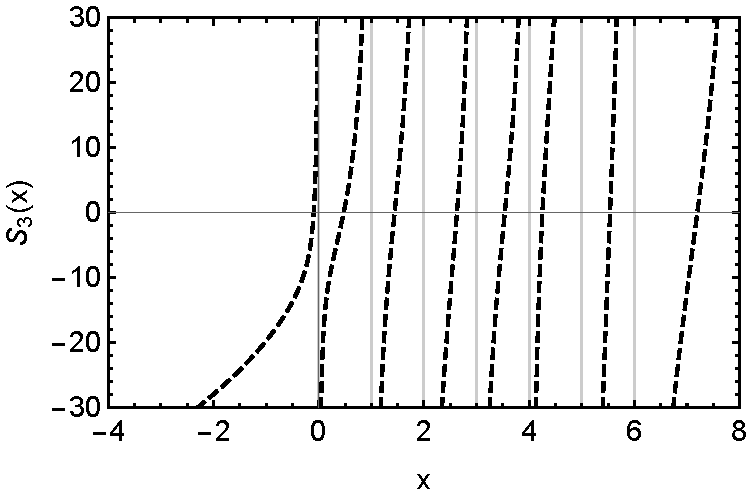
\includegraphics[width=.8\columnwidth]{figure/S3.pdf}
\caption{The function $S_3(x)$ defined in eq.~\eqref{eqn:S3}.\label{fig:S3}}
\end{figure}

\subsubsection{$d=2$}
Using eq.~\eqref{eqn:C 2} in eq.~\eqref{eqn:quantization} we find
\begin{multline}
-\frac{m \log (a_0\Lambda)}{2 \pi }-\frac{1}{L^2}\sum_{\vec{q}}^\Lambda \frac { 1 } { E - \frac{\vec{q}^2}{m} }=0\\
\implies
\frac{2}{\pi}\log (pa_0)+\frac{2}{\pi}\log(\Lambda/p)=-\frac{4}{mL^2}\sum_{\vec{q}}^\Lambda \frac { 1 } { E - \frac{\vec{q}^2}{m} }\ .
\end{multline}
Now as in the previous section, we use the phase shift relation of eq.~\eqref{eqn:phase shifts}, and after a little manipulation, We find
\begin{equation}
\cot \delta(p)=\frac{1}{\pi^2}S_2\left(\left(\frac{pL}{2\pi}\right)^2\right)+\frac{2}{\pi}\log\left(\frac{pL}{2\pi}\right)\ ,
\end{equation}
where
\begin{equation}\label{eqn:S2}
S_2(x)\equiv\sum_{\vec{n}}^{\Lambda'} \frac { 1 } { \vec{n}^2 -x}-2\pi\log\left(\Lambda'\right)\ ,
\end{equation}
where $\Lambda'=\frac{\Lambda L}{2\pi}$.
Here $\vec{n}=(n_x,n_y)$ is a doublet of integers and the limit $\Lambda'\to\infty$ is implicit.   \autoref{fig:S2} shows the functional form of eq.~\eqref{eqn:S2}.
\begin{figure}
\center
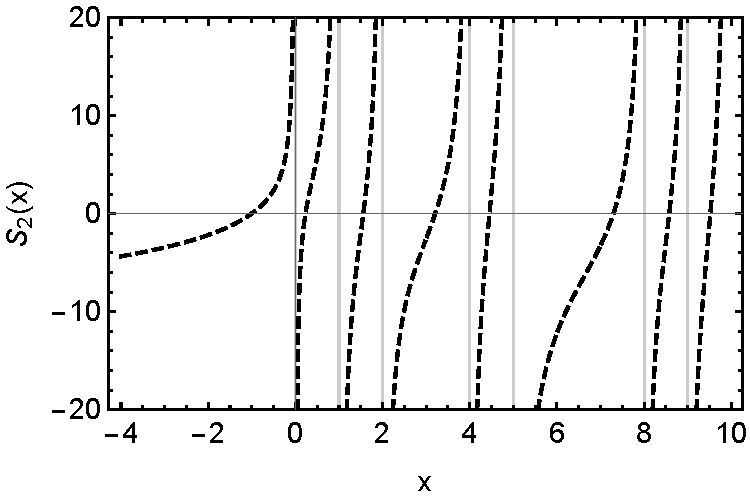
\includegraphics[width=.8\columnwidth]{figure/S2.pdf}
\caption{The function $S_2(x)$ defined in eq.~\eqref{eqn:S2}.\label{fig:S2}}
\end{figure}

\subsubsection{$d=1$}
Using eq.~\eqref{eqn:C 1} in eq.~\eqref{eqn:quantization} We find
\begin{equation}
-\frac{ma_0}{2}-\frac{1}{L}\sum_{\vec{q}} \frac { 1 } { E - \frac{\vec{q}^2}{m} }=0
\implies
p a_0=-\frac{2p}{mL}\sum_{\vec{q}} \frac { 1 } { E - \frac{\vec{q}^2}{m} }\ .
\end{equation}
Again, we use eq.~\eqref{eqn:phase shifts}, and after a little manipulation, we get
\begin{align}
\frac{1}{p}\cot\delta_0(p)=a_0&=\frac{L}{2\pi^2}\sum_{n=-\infty}^{\infty} \frac { 1 } { n^2 -\left(\frac{pL}{2\pi}\right)^2}\\
 &\equiv\frac{L}{2\pi^2} S_1\left(\left(\frac{pL}{2\pi^2}\right)^2\right)\ ,
\end{align}
where
\begin{equation}\label{eqn:S1}
S_1(x)\equiv\sum_{n=-\infty}^{\infty} \frac { 1 } { n^2 -x}=-\pi\frac{\cot(\pi\sqrt{x})}{\sqrt{x}}\ .
\end{equation}
This function is valid for $x$ both positive and negative, and is shown in \autoref{fig:S1}.
\begin{figure}
\center
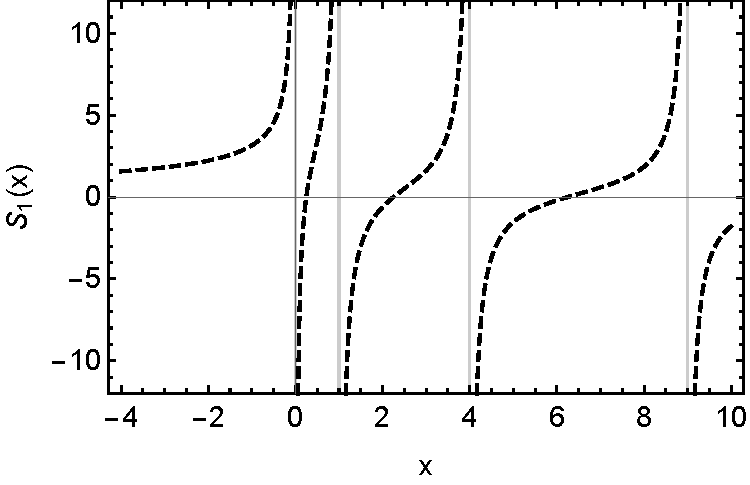
\includegraphics[width=.8\columnwidth]{figure/S1.pdf}
\caption{The function $S_1(x)$ defined in Eq.\eqref{eqn:S1}.\label{fig:S1}}
\end{figure}

\begin{itemize}
\item Bound state in $L\to\infty$ limit\todo{needs work}
\item Scattering states in $L\to\infty$\todo{needs work}
\end{itemize}


\section{Recap}
My findings for L\"uscher's formula in the different dimensions are
\begin{align}
p\cot \delta(p)&=\frac{1}{\pi L}S_3\left(\left(\frac{pL}{2\pi}\right)^2\right)&(d=3)\\
\cot \delta(p)&=\frac{1}{\pi^2}S_2\left(\left(\frac{pL}{2\pi}\right)^2\right) +\frac{2}{\pi}\log\left(\frac{pL}{2\pi}\right)&(d=2)\\
\frac{1}{p}\cot\delta_0(p)&= 
\frac{L}{2\pi^2} S_1\left(\left(\frac{pL}{2\pi}\right)^2\right)
 &(d=1)
\end{align}
where $S_3(x)$, $S_2(x)$, and $S_1(x)$ are given by Eqs.~\eqref{eqn:S3},~\eqref{eqn:S2}, and~\eqref{eqn:S1}, respectively.


%\subsection{}

%\newpage
%\appendix

%\clearpage
\bibliographystyle{h-physrev3}
\bibliography{master}

\end{document}  
